\chapter{Writing Assignment Expectations}

\section{General expectations}

The mathematical writing you do for this class needs to be done with sentences and paragraphs (even when it appears that the question just asks you to do some algebra.)  However, in mathematical writing we do not just use words; we use graphs, symbols and numbers mixed in with the words.  Look in your textbook at the mix of these 4 elements. The writing you do in this class must have sentences and paragraphs, but the minimal requirement for the writing in this class is that you have at least one other representation.  In other words, you have to have at least 2 of the 4 representations of mathematics described below and one of those representations must include sentences and paragraphs.
 There are 4 ways to represents mathematical ideas:  {\bf{graphically}}, {\bf{symbolically}}, {\bf{tabularly}} and {\bf{verbally}}.  For example, let us first consider a line.  We can represent the line {\bf{graphically}} like this $\ldots$
\begin{figure}[h]
	\centering
		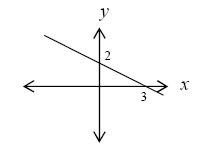
\includegraphics{TeXGraphics/ExpectationsFigurea.jpg}
	\label{Expectations}
\end{figure}

$\ldots$ or {\bf{symbolically}} like this $\ldots$
 $$2x + 3y = 6$$
 
$\ldots$ or we can find a list of points on that line {\bf{tabularly}} like this $\ldots$
 $$\begin{array}{|c|c|}
 \hline
   x & y  \\ \hline
   0 & 2  \\ \hline
   3 & 0  \\ \hline
   1 & {{\textstyle{4 \over 3}}}  \\ \hline
   {{\textstyle{3 \over 2}}} & 1  \\ \hline
    {- 3} & 4 \\ \hline
 \end{array}$$

$\ldots$ or we can describe the line {\bf{verbally}} like this $\ldots$
 \begin{quote}{This line has a slope of $ - {2 \over 3},$ an $x$-intercept of $x = 3$ and a $y$-intercept of $y = 2$.}\end{quote}

{\bf{Graphical}} representations might include the usual type of graphs, diagrams, pictures, etc.  {\bf{Symbolic}} representations might include algebraic operations, equations, evaluation of formulas, etc.  {\bf{Tabular}} representations might include lists of data points, calculations, numerical investigations, etc.  {\bf{Verbal}} descriptions include sentences and paragraphs but would also include verbal annotations of graphs, symbols and tables.

 It is your responsibility to develop a satisfactory method of writing mathematics.  It may take a few assignments for everyone to understand what is expected but I will provide you with examples of good (and bad) writing during the first couple of weeks of class to help you understand.  The writing assignments that are due each week are relatively low risk, i.e., the score for each individual assignment is a small part of your grade and you have a chance to make up these assignments.  However, one purpose of the daily writing assignments is to prepare you to do well on the writing that will be on the exams where the risk is higher.  So use the daily writings to work on your style and presentation.
 
	\section{Grading Rubric}
	 
Each writing assignment is worth 4 points.
\begin{itemize}
\item {\bf{1 point}}:  The mathematics is correct with only minor arithmetic or notational errors.  The mathematical language, notation and symbols are correct and appropriate.
\item  {\bf{1 point}}:  The writing and organization is well done with only minor grammar or spelling errors.  The writing is well organized around a central theme and flows well.  
\item  {\bf{1 point}}:  The writing answered the questions asked and there is no "fluff".
\item  {\bf{1 point}}:  Sufficient evidence is given to support the answer (i.e., graphical, symbolic, tabular and verbal representations).  Examples are used to elaborate on and to clarify the concepts discussed.  
\end{itemize}
 It is possible to get a 2.5 for a grade.  This might mean the writing had problems (loss of 1 point) and you had some evidence but could have had more (loss of 0.5 of a point).  I will try to give you comments that will help you understand why you lost points.  Of course, not all writing requires examples \emph{and} algebra \emph{and}graphs \emph{and}numerical calculations, but you should try to include these whenever appropriate.  These constitute evidence that you understand the concept fully and support the claims you make in the writing.

  \section{ Expectations of specific question types}

\begin{description}
\item[Compare and contrast] You will often be asked to compare and contrast two 
concepts.  To compare and contrast you need to describe the ways in which the 
concepts are the same (compare) and the ways in which the concepts are different 
(contrast).  Sometimes making a side-by-side list of features of the 2 concepts 
will help you organize your work. You must have sentences that start with 
"These concepts are alike because..." and "These concepts are different because...".  A description of each concept without connection to the other is unnecessary and does not satisfy the requirements of this type of question.  
\item[Annotated example]  An annotated example has sentences that explain each step of the calculation.  On way to write a nice annotated example is first to do the mathematics.  Include a reference number at the end of each line, like this.
 $$\begin{array}{rclr}
  f(x)& = &\left( {x - 2} \right)^3 \left( {x + 3} \right)^2  & (1) \\ 
  f'(x)& =& 3\left( {x - 2} \right)^2 \left( {x + 3} \right)^2  + 2\left( {x - 2} \right)^3 \left( {x + 3} \right) & (2) \\ 
   &= &5\left( {x - 2} \right)^2 \left( {x + 3} \right)\left( {x + 1} \right) &  (3) 
\end{array} 
$$

Now, write a paragraph about the work you did.  You can easily refer to specific work by using the reference numbers.  "We took the function (1) and found the derivative (2) by using the product rule.  Equation (3) is a factored version of (2)."  Tell the reader what you did, what rules or theorems you used, and anything else that will help him or her understand the results.  Write actively and use first person plural.  Notice that I did not include every single excruciating detail of the calculus and algebra.  Remember that what you turn in must be a final product so you can choose the most important steps to include.
\item[Concept map]  A concept map is a diagram of your own design that shows the interrelationships of a set of concepts.  Sentences describing the relationships and other aspects of the concepts are included in the map.  You can include any helpful information such as comparisons, contrasts, extensions, generalizations, parallels, etc.  Remember that the concept maps fall under the category of writing, so there has to be a significant amount of writing in the map even if it is not in the standard paragraph form of an essay.
\item[Generalization]  When asked to generalize you need to describe what happens in the general case.  For example, we know that the solution to $x^2 - 4 = 0$ is $x = 2$ and $x = -2$.  A generalization of this is that the solution to $x^2 - k = 0$ is $$
x = \sqrt k 
$$
 and $$
x =  - \sqrt k 
.$$
  To find a generalization, I used an unknown constant in the place of a number and described the solution in that general case.  Sometimes to generalize we see what happens in the $n$th case.  We know that 
$ax + b = 0$ has at most 1 real solution and $ax^2 + bx + c = 0$ has at most 2 real solutions.  To generalize, we might try to show that a polynomial equation of degree $n$ has at most $n$ real solutions.
\item [True or false]  Some of the questions ask you to determine if a statement is always true or not always true.  If it is always true, you need to provide an argument to justify this claim.  If it is not always true, you should provide an example and a counterexample.  If the statement is never true, you need to provide an argument to justify this claim.
\end{description}

 \section{References}

These expectations was developed using the ideas in Jerry Stonewater's writing \cite{SJ}.
  
